
\def\scl{0.3}%scaling factor of the picture
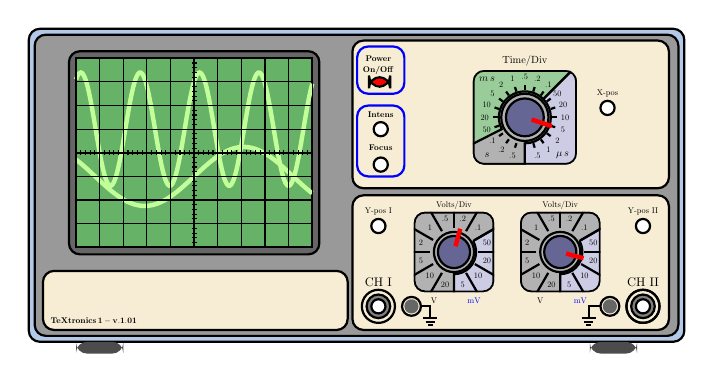
\begin{tikzpicture}[
  scale=\scl,
  controlpanels/.style={yellow!30!brown!20!,rounded corners,draw=black,thick},
  screen/.style={green!50!black!60!,draw=black,thick},
  trace/.style={green!60!yellow!40!, ultra thick},
  smallbutton/.style={white,draw=black, thick},
  axes/.style={thick}]
  \fill[green!30!blue!30!,rounded corners,draw=black,thick](0,0)
    rectangle (27.75,13.25);
  \fill[fill=black!40!,draw=black,thick,rounded corners](0.25,0.25)
    rectangle (27.5,13.00);
  % Screen, centered around the origin then shifted for easy plotting
  \begin{scope}[xshift=7cm,yshift=8cm,samples=150]
    \fill[black!60!,rounded corners,draw=black,thick](-5.3,-4.3)
      rectangle (5.3,4.3);
    \fill[screen] (-5.0,-4.0) rectangle (5.0,4.0);
    \draw[trace] plot(\x,{1+2.4*sin((2.5*\x +1) r)}); % r for radians...
    \draw[trace] plot(\x,{-1+1.25*sin((0.75*\x) r});
    \draw[thin] (-5.0,-4.0) grid (5.0,4.0);
    \draw[axes] (-5,0)--(5,0); % Time axis
    \draw[axes] (0,-4)--(0,4);
    \foreach \i in {-4.8,-4.6,...,4.8} \draw (\i,-0.1)--(\i,0.1);
    \foreach \i in {-3.8,-3.6,...,3.8} \draw (-0.1,\i)--(0.1,\i);
  \end{scope}
  % Feet
  \fill[black!70!,rounded corners,xshift=2cm] (0,-.5) rectangle (2,0);
  \fill[black!70!,rounded corners,xshift=23.75cm] (0,-.5) rectangle (2,0);
  % Lower left panel
  \fill[controlpanels] (0.6,0.5) rectangle (13.5,3.0);
  \path (0.8,0.9) node[scale=\scl,right]{$\mathbf{TeXtronics\,1 - v.1.01}$};
  % Lower right panel
  \fill[controlpanels] (13.7,0.5) rectangle (27.1,6.2);
  %Channels
  % CH I
  \draw[thick] (14.8,1.5) circle (0.7cm);
  \fill[gray,draw=black,thick] (14.8,1.5) circle (0.5cm);
  \fill[white,draw=black,thick] (14.8,1.5) circle (0.3cm);
  \node[scale={1.5*\scl}] at (14.8,2.5) {CH I};
  \draw[thick] (16.2,1.5) circle (0.4cm);
  \fill[black!60!] (16.2,1.5) circle (0.3cm);
  \draw[thick] (16.6,1.5) --(17,1.5)--(17,1.0);
  \draw[thick] (16.7,1.0)--(17.3,1.0);
  \draw[thick] (16.8,0.85)--(17.2,0.85);
  \draw[thick] (16.9,0.70)--(17.1,0.70);
  \draw[thick] (26.0,1.5) circle (0.7cm);
  % CH II
  \fill[gray,draw=black,thick] (26,1.5) circle (0.5cm);
  \fill[white,draw=black,thick] (26,1.5) circle (0.3cm);
  \node[scale={1.5*\scl}] at (26,2.5) {CH II};
  \draw[thick] (24.6,1.5) circle (0.4cm);
  \fill[black!60!] (24.6,1.5) circle (0.3cm);
  \draw[thick] (24.2,1.5) --(23.7,1.5)--(23.7,1.0);
  \draw[thick] (23.4,1.0)--(24.0,1.0);
  \draw[thick] (23.5,0.85)--(23.9,0.85);
  \draw[thick] (23.6,0.70)--(23.8,0.70);
  \draw[thick] (26.0,1.5) circle (0.7cm);
  % Y-pos
  \fill[smallbutton] (14.8,4.9) circle (0.3cm);
  \node[scale={\scl}] at (14.8,5.5) {Y-pos I};
  \fill[smallbutton] (26.0,4.9) circle (0.3cm);
  \node[scale={\scl}] at (26.0,5.5) {Y-pos II};
  % Volt/div the foreach loop draws the two buttons
  \foreach \i / \b in {18/75,22.5/345}{
  %Second parameter of the loop is the angle of the index mark 
  \begin{scope}[xshift=\i cm,yshift=3.8cm,scale=0.85]
    \node[scale=\scl] at (0,2.3) {Volts/Div};
    \node[scale=\scl,black] at (-1,-2.4) {V};
    \node[scale=\scl,blue]  at (1,-2.4) {mV};
    \clip[rounded corners] (-2,-2) rectangle (2,2);
    \fill[black!30!,rounded corners,draw=black,thick] (-2,-2)
      rectangle (2,2);
    \fill[blue!50!black!20!,draw=black,thick]
      (30:1.1)--(30:3)--(3,-3)--(-90:3)--(-90:1.1) arc (-90:30:1.1);
    \draw[very thick,rounded corners](-2,-2) rectangle (2,2);
    \draw[thick] (0,0) circle (1.0);
    \foreach \i in {0,30,...,330}
      \draw[thick] (\i:1.2)--(\i:2.5);
    \foreach \i/\j in {15/50,45/.1,75/.2,105/.5,135/1,165/2,195/5,225/10,
      255/20,285/5,315/10,345/20} \node[scale=\scl,black] at (\i:1.7) {\j};
    \fill[blue!30!black!60!,draw=black,thick] (0,0) circle (0.8cm);
    % Here you set the right Volts/Div button
    \draw[ultra thick,red] (\b:0.3)--(\b:1.2);
  \end{scope}}
% Upper right panel
  \fill[controlpanels] (13.7,6.5) rectangle (27.1,12.75);
  %On-Off button
  \draw[rounded corners,thick,blue] (13.9,10.5) rectangle (15.9,12.5);
  \fill[fill=red,draw=black,thick,rounded corners] (14.4,10.8) rectangle (15.3,11.2);
  \node[scale=\scl] at (14.8,12) {\textbf{Power}};
  \node[scale=\scl] at (14.8,11.5) {\textbf{On/Off}};
  % Focus-Intensity buttons
  \draw[rounded corners,thick,blue] (13.9,7.0) rectangle (15.9,10.0);
  \fill[smallbutton] (14.9,7.5) circle (0.3cm);
  \node[scale=\scl] at (14.9,8.2) {\textbf{Focus}};
  \fill[smallbutton] (14.9,9) circle (0.3cm);
  \node[scale=\scl] at (14.9,9.6) {\textbf{Intens}};
  % X-pos
  \fill[smallbutton] (24.5,9.9) circle (0.3cm);
  \node[scale={\scl}] at (24.5,10.5) {X-pos};
  % Time/Div
  \begin{scope}[xshift=21cm,yshift=9.5cm,scale=1]
    \node[scale={1.25*\scl}]  at (0,2.4) {Time/Div};
    \clip[rounded corners] (-2.2,-2) rectangle (2.2,2);
    \fill[black!30!,rounded corners,draw=black,thick] (-2.2,-2) rectangle (2.2,2);
    \fill[blue!50!black!20!,draw=black,thick]
      (45:1.1)--(45:3)--(3,-3)--(-90:3)--(-90:1.1) arc (-90:45:1.1);
    \fill[green!50!black!40!,draw=black,thick]
      (45:1.1)--(45:3) arc(45:207:3) --(207:1.1) arc (207:45:1.1);
    \draw[very thick,rounded corners](-2.2,-2) rectangle (2.2,2);
    \node[scale={1.25*\scl}] at (-1.6,-1.6) {$s$};
    \node[scale={1.25*\scl}] at (1.6,-1.6) {$\mu{}\,s$};
    \node[scale={1.25*\scl}] at (-1.6,1.6) {$m\,s$};
    \draw[thick] (0,0) circle (1.0);
    \foreach \i in {-72,-54,...,262} \draw[thick] (\i:1.15)--(\i:1.35);
    \foreach \i/\j in {-72/.5,-54/1,-36/2,-18/5,0/10,18/20,36/50,54/.1,72/.2,90/.5,
      108/1,126/2,144/5,162/10,180/20,198/50,216/.1,234/.2,252/.5}
      \node[scale=\scl,black] at (\i:1.7){\j};
    \fill[blue!30!black!60!,draw=black,thick] (0,0) circle (0.8cm);
    % Here you set the Time/Div button
    \draw[ultra thick,red] (-18:0.3)--(-18:1.2);	
    % X-pos
  \end{scope}
\end{tikzpicture}